\chapter{Exercise 09}
\extitle{Practicing Regularized Logistic Regression}
%%******************************************************************************%
%                                                                              %
%                                 Interlude                                    %
%                         for Machine Learning module                          %
%                                                                              %
%******************************************************************************%

% ============================================== %
\section*{Interlude - Lost in Overfitting}
% ---------------------------------------------- %

The two previous exercises lead you, dear reader, to a very dangerous territory: the realm of \textbf{overfitting}.\\
You did not see it coming but now, you are in a bad situation...\\
\\
By increasing the polynomial degree of your model, you increased its \textbf{complexity}.  
Is it wrong?
Not always.
Some models are indeed very complex because the relationships they represent are very complex as well.\\
\\
But, if you look at the plots for the previous exercise's \textit{best model}, you should feel that something is wrong...\\
\\
% ============================================== %
\section*{Interlude - Something is rotten in the state of our model...}
% ---------------------------------------------- %
Take a look at the following plot. 

\begin{figure}[!h]
    \centering
    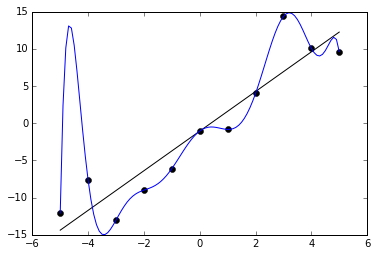
\includegraphics[scale=0.6]{assets/overfitt.png}
    \caption{Overfitting hypothesis}
\end{figure}

You can see that the prediction line fits each data point perfectly, but completely misses out on capturing the relationship between $x$ and $y$ properly.
And now, if we add some brand new data points to the dataset, we see that the predictions on those new examples are way off.

\begin{figure}[!h]
    \centering
    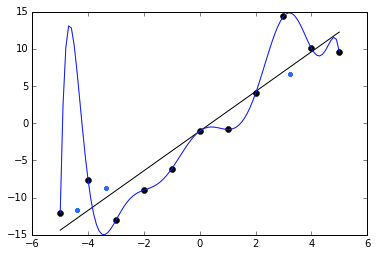
\includegraphics[scale=0.6]{assets/overfitt_with_dots.png}
    \caption{Generalization errors resulting from overfitting}
\end{figure}
This situation is called overfitting, because the model is doing an excessively good job at fitting the data.
It is literally bending over backward to account for the data's mini details.
But most of the data's irregularities are just noise, and they should in fact be ignored.
So because the model overfits, it can't generalize to new data.

% ============================================== %
\section*{Interlude - The training set, the test set, and the happy data scientist}
% ---------------------------------------------- %
To be able to detect overfitting, \textbf{you should always evaluate your model on new data}.\\
\\
New data means, data that your model hasn't seen during training.\\
\\
It's the only way to make sure your model isn't \textit{recalling}.
To do so, now and forever, you must always divide your dataset in (at least) two parts: one for the training, and one for the evaluation of your model.
%\newpage
\turnindir{ex09}
\exnumber{09}
\exfiles{solar\_system\_census.py, benchmark\_train.py,  models.[csv/yml/pickle]}
\exforbidden{sklearn}
\makeheaderfilesforbidden

% ================================= %
\section*{Objective}
% --------------------------------- %
It's training time!
Let's practice our updated Logistic Regression with polynomial models.
% ================================= %
\section*{Introduction}
% --------------------------------- %
You have already used the dataset \texttt{solar\_system\_census.csv} and \texttt{solar\_system\_census\_planets.csv}.
\begin{itemize}
	\item The dataset is divided in two files which can be found in the \texttt{resources} folder: \texttt{solar\_system\_census.csv} and \texttt{solar\_system\_census\_planets.csv}.
	\item The first file contains biometric information such as the height, weight, and bone density of several Solar System citizens.
	\item The second file contains the homeland of each citizen, indicated by its Space Zipcode representation (i.e. one number for each planet... :)).  
\end{itemize}

As you should know, Solar citizens come from four registered areas (zipcodes): 

\begin{itemize}
	\item The flying cities of Venus ($0$), 
	\item United Nations of Earth ($1$), 
	\item Mars Republic ($2$), 
	\item The Asteroids' Belt colonies ($3$).
\end{itemize}

% ================================= %
\section*{Instructions}
% --------------------------------- %
% ================================= %
\subsection*{Split the Data}
% --------------------------------- %

Take your \texttt{solar\_system\_census.csv} dataset and split it in a \textbf{training set}, a \textbf{cross-validation set}
and  a \textbf{test set}.

% ================================= %
\subsection*{Training and benchmark}
% --------------------------------- %
One part of your submission will be find in \texttt{benchmark\_train.py} and \texttt{models.[csv/yml/pickle]} files.
You have to:
\begin{itemize}
  \item Train different regularized logistic regression models with a polynomial hypothesis of \textbf{degree 3}.
        The models will be trained with different $\lambda$ values, ranging from $0$ to $1$.
        Use one-vs-all method.
  \item Evaluate the \textbf{f1 score} of each of the models on the cross-validation set.
        You can use the \texttt{f1\_score\_} function that you wrote in the \texttt{ex11} of \texttt{module08}.
  \item Save the different models into a \texttt{models.[csv/yml/pickle]}.
\end{itemize}

% ================================= %
\subsection*{Solar system census program}
% --------------------------------- %
The second and last part of your submission is in \texttt{solar\_system\_census.py}. You have to:
\begin{itemize}
  \item Loads the differents models from \texttt{models.[csv/yml/pickle]} and train from scratch only the best one on a training set.
  \item Visualize the performance of the different models with a bar plot showing the score of the models given their $\lambda$ value.
  \item Print the \textbf{f1 score} of all the models calculated on the test set.
  \item Visualize the target values and the predicted values of the best model on the same scatterplot. Make some effort to have a readable figure.
\end{itemize}

\info{For the second script \texttt{solar\_system\_census.py}, only a train and test set are necessary as one is simply looking to the performance.}
